\textbf{Convention:} To any product, we associate morphisms denoted by $\pi_i$,
where $i$ is an index of the product component we are projecting to, or is the
component itself. For example, for $A\times B$ we have $\pi_A:A\times B\rightarrow A$, for
$A^n$ we have $\pi_i:A^n\rightarrow A$ with $i\in\llbracket1,n\rrbracket$, for $\prod_{i\in I} A_i$
we have $\pi_{i_0}:\prod_{i\in I} A_i\rightarrow A_{i_0}$ for $i_0\in I$.
Similarly, we introduce a notion $i$ for morphisms associated to coproducts.
A projection on the tangent space is always associated to $T_xM\times (T_xM)^\bot$.

\vspace{2ex}
\textbf{Convention:} Let $\{w_i\}_i$ be a family of some kind of objects.We
write a row of those objects as $(w_i)$ and column as $(w^i)$. We will use
matrix multiplication notion to shorten equations, even when dealing with things
that might not be scalars. For example, a basis change formula from basis
$(w_i)$ to a basis $(u_i)$ with a matrix $P$ is denoted by $(u_i)=(w_i)P$. If
we have two function $f,g$ defined on $X$ and we have $a,b\in X$ then we may write
\[\left(\begin{array}{c}f\\g\end{array}\right)(a\;\;b)=\left(\begin{array}{cc}f(a)&f(b)\\g(a)&g(b)\end{array}\right)\quad\quad f\left(\begin{array}{c}a\\b\end{array}\right)=\left(\begin{array}{c}f(a)\\f(b)\end{array}\right)\]
Often this way of writing equations compactifies not only notions but also proofs,
as you will see in Section 7, by using substitutions. Although, I switch later
in that section to Einstein's convention, because it eases permutations of
sums and regrouping of coordinates.

\subsection{Measure theory}
Geometric Measure Theory is based upon Radon measure theory, where the notion of
outer measure is obligatory. We consider that any set can be measured.

\vspace{1ex}
\textbf{Definition:} \textit{An \textbf{outer measure} on $X$ is a set function on $X$ with
values in $[0,\infty]$ with
\begin{itemize}
    \item $\mu(\varnothing)=0$
    \item $E\subseteq\bigcup_{h\in\mathbb{N}}E_h\quad\Rightarrow\quad\mu(E)\leq\sum_{h\in\mathbb{N}}\mu(E_h)$
\end{itemize}
}

\vspace{2ex}
\textbf{Carathéodory's theorem:} \textit{If $\mu$ is an outer measure on $X$ and $\mathcal
M(\mu)$ is the family of those $E\subseteq X$ such that
\[\mu(F)=\mu(E\cap F)+\mu(F\setminus E),\quad\quad\forall F\subseteq X\]
then $\mathcal M(\mu)$ is a $\sigma$-algebra and $\mu$ is a measure on $\mathcal
M(\mu)$.}

\vspace{2ex}
A proof can be found on pages 8-9 of \cite{maggi}.

\vspace{2ex}
\textbf{Definition:} \textit{$\mu$ is a \textbf{Borel measure} on a topological space $X$
if it is an outer measure on $X$ such that $\mathcal B(X)\subseteq\mathcal M(\mu)$.}

\vspace{2ex}
\textbf{Definition:} \textit{A measure $\mu$ is said to be \textbf{absolutely continuous
with respect to} measure $\lambda$ if for any set $A$, $\lambda(A)=0$
implies $\mu(A)=0$ and we write it $\mu << \lambda$.}

\vspace{2ex}
\textbf{Definition:} \textit{We say that a Borel measure $\mu$ is \textbf{regular} if
for every $F\subseteq X$ there exists a Borel set $E\in\mathcal B(X)$ such that
\[F\subseteq E,\quad\quad\quad\quad\quad\quad\mu(F)=\mu(E)\]}

\vspace{2ex}
\textbf{Definition:} \textit{An outer measure $\mu$ on $X$ is \textbf{locally finite} if
$\mu(K)<\infty$ for every compact set $K\subseteq X$.}

\vspace{2ex}
\textbf{Definition:} \textit{An outer measure $\mu$ is a \textbf{Radon measure} on a
topological space if it is locally finite, Borel regular measure on $X$.}

\vspace{2ex}
\textbf{Property of Radon measures on $\mathbb{R}^n$:} \textit{If $\mu$ is a Radon
measure on $\mathbb{R}^n$, then
\[
    \mu(E)=\inf\{\mu(A)\,|\,E\subseteq A,\,A\textnormal{ is open}\}
          =\sup\{\mu(K)\,|\,K\subseteq E,\,K\textnormal{ is compact}\}
\]}

\vspace{2ex}
Those are only top-level results. While this theory incorporates many more
profound statements, I've avoided them here to maintain the holistic picture I aim 
to present and not to have just another copy of an already existing book. This
necessarily means sacrificing some depth, as I have not included few necessary 
proofs and results.

\subsection{Analysis}
Geometric measure theory relies on several profound and not-trivial results
established within metric spaces or $\mathbb{R}^n$. This foundational
properties, which I adapted with minor modifications or gave direct
generalisations, are primarily sourced from "Measure theory and fine properties
of functions".

\vspace{2ex}
For a ball $B=B(x, r)$ of center $x$ and radius $r$ we shall note $\prescript{\epsilon}{}B
=B(x, (1+\epsilon)r)$ for every $\epsilon>0$. I chose the prefix notation to
avoid confusion with set power and Minkowski product.

\vspace{1ex}
\textbf{Vitali's covering lemma:} \textit{
Let $\mathcal{F}$ be any collection of non-degenerated closed balls in a metric
space $X$ with
\[ \sup\{\text{diam}\,B\,|\, B\in\mathcal{F}\}<\infty \]
Then for every $\epsilon>1$ there exists a countable family $\mathcal{G}$ of
disjoint balls in $\mathcal{F}$ such that
\[\bigcup_{B\in\mathcal{F}}B\subseteq\bigcup_{B\in\mathcal{G}}\prescript{2\epsilon}{}B\]}

\vspace{1ex}
\textbf{Proof:}
Set $D=\sup\{\text{diam}\,B\,|\,B\in \mathcal{F}\}$. Set
\[\mathcal{F}_j=\left\{B\in\mathcal{F}\,|\,\frac{D}{\epsilon^j}<\text{diam}\,B\leq\frac{D}{\epsilon^{j-1}}\right\},\quad j=1,2,\ldots\]
We define $\mathcal{G}_j\subseteq\mathcal{F}_j$ as follows
\begin{itemize}
    \item Let $\mathcal{G}_1$ be any maximal disjoint collection of balls in
        $\mathcal{F}_1$.

    \item Assuming $\mathcal{G}_1,\ldots,\mathcal{G}_{k-1}$ have been selected,
        we chose $\mathcal{G}_k$ to be any maximal disjoint subcollection of
        \[ \{B\in\mathcal{F}_k\,|\,B\cap B'=\varnothing\text{ for all }B'\in\bigcup_{j=1}^{k-1}\mathcal{G}_j\}\]
\end{itemize}
They exist by Zorn's Lemma. Finally, define $\mathcal{G}=\bigcup_{j\in\mathbb{N}^*}\mathcal{G}_j$
a collection of disjoint balls and $\mathcal{G}\subseteq\mathcal{F}$.

\vspace{1ex}
Proving that for each ball $B\in\mathcal{F}$, there exists a ball $B'\in\mathcal{G}$
such that $B\cap B'\neq\varnothing$ and $B\subseteq\prescript{\epsilon}{}B'$. Fix
$B\in\mathcal{F}$, there exists and index $j$ such that $B\in\mathcal{F}_j$ and
by maximality of $\mathcal{G}_k$ there exists a ball $B'\in\bigcup_{k=1}^j
\mathcal{G}_k$ with $B\cap B'\neq\varnothing$. But $\text{diam}\,B'>\frac{D}{\epsilon^j}$
and $\text{diam}\,B\leq\frac{D}{\epsilon^{j-1}}$; so that
\[ \text{diam}\,B\leq \frac{D}{\epsilon^{j-1}} < \epsilon\text{diam}\,B'\]
Thus $B\subseteq\prescript{2\epsilon}{}B'$.
\begin{center}
    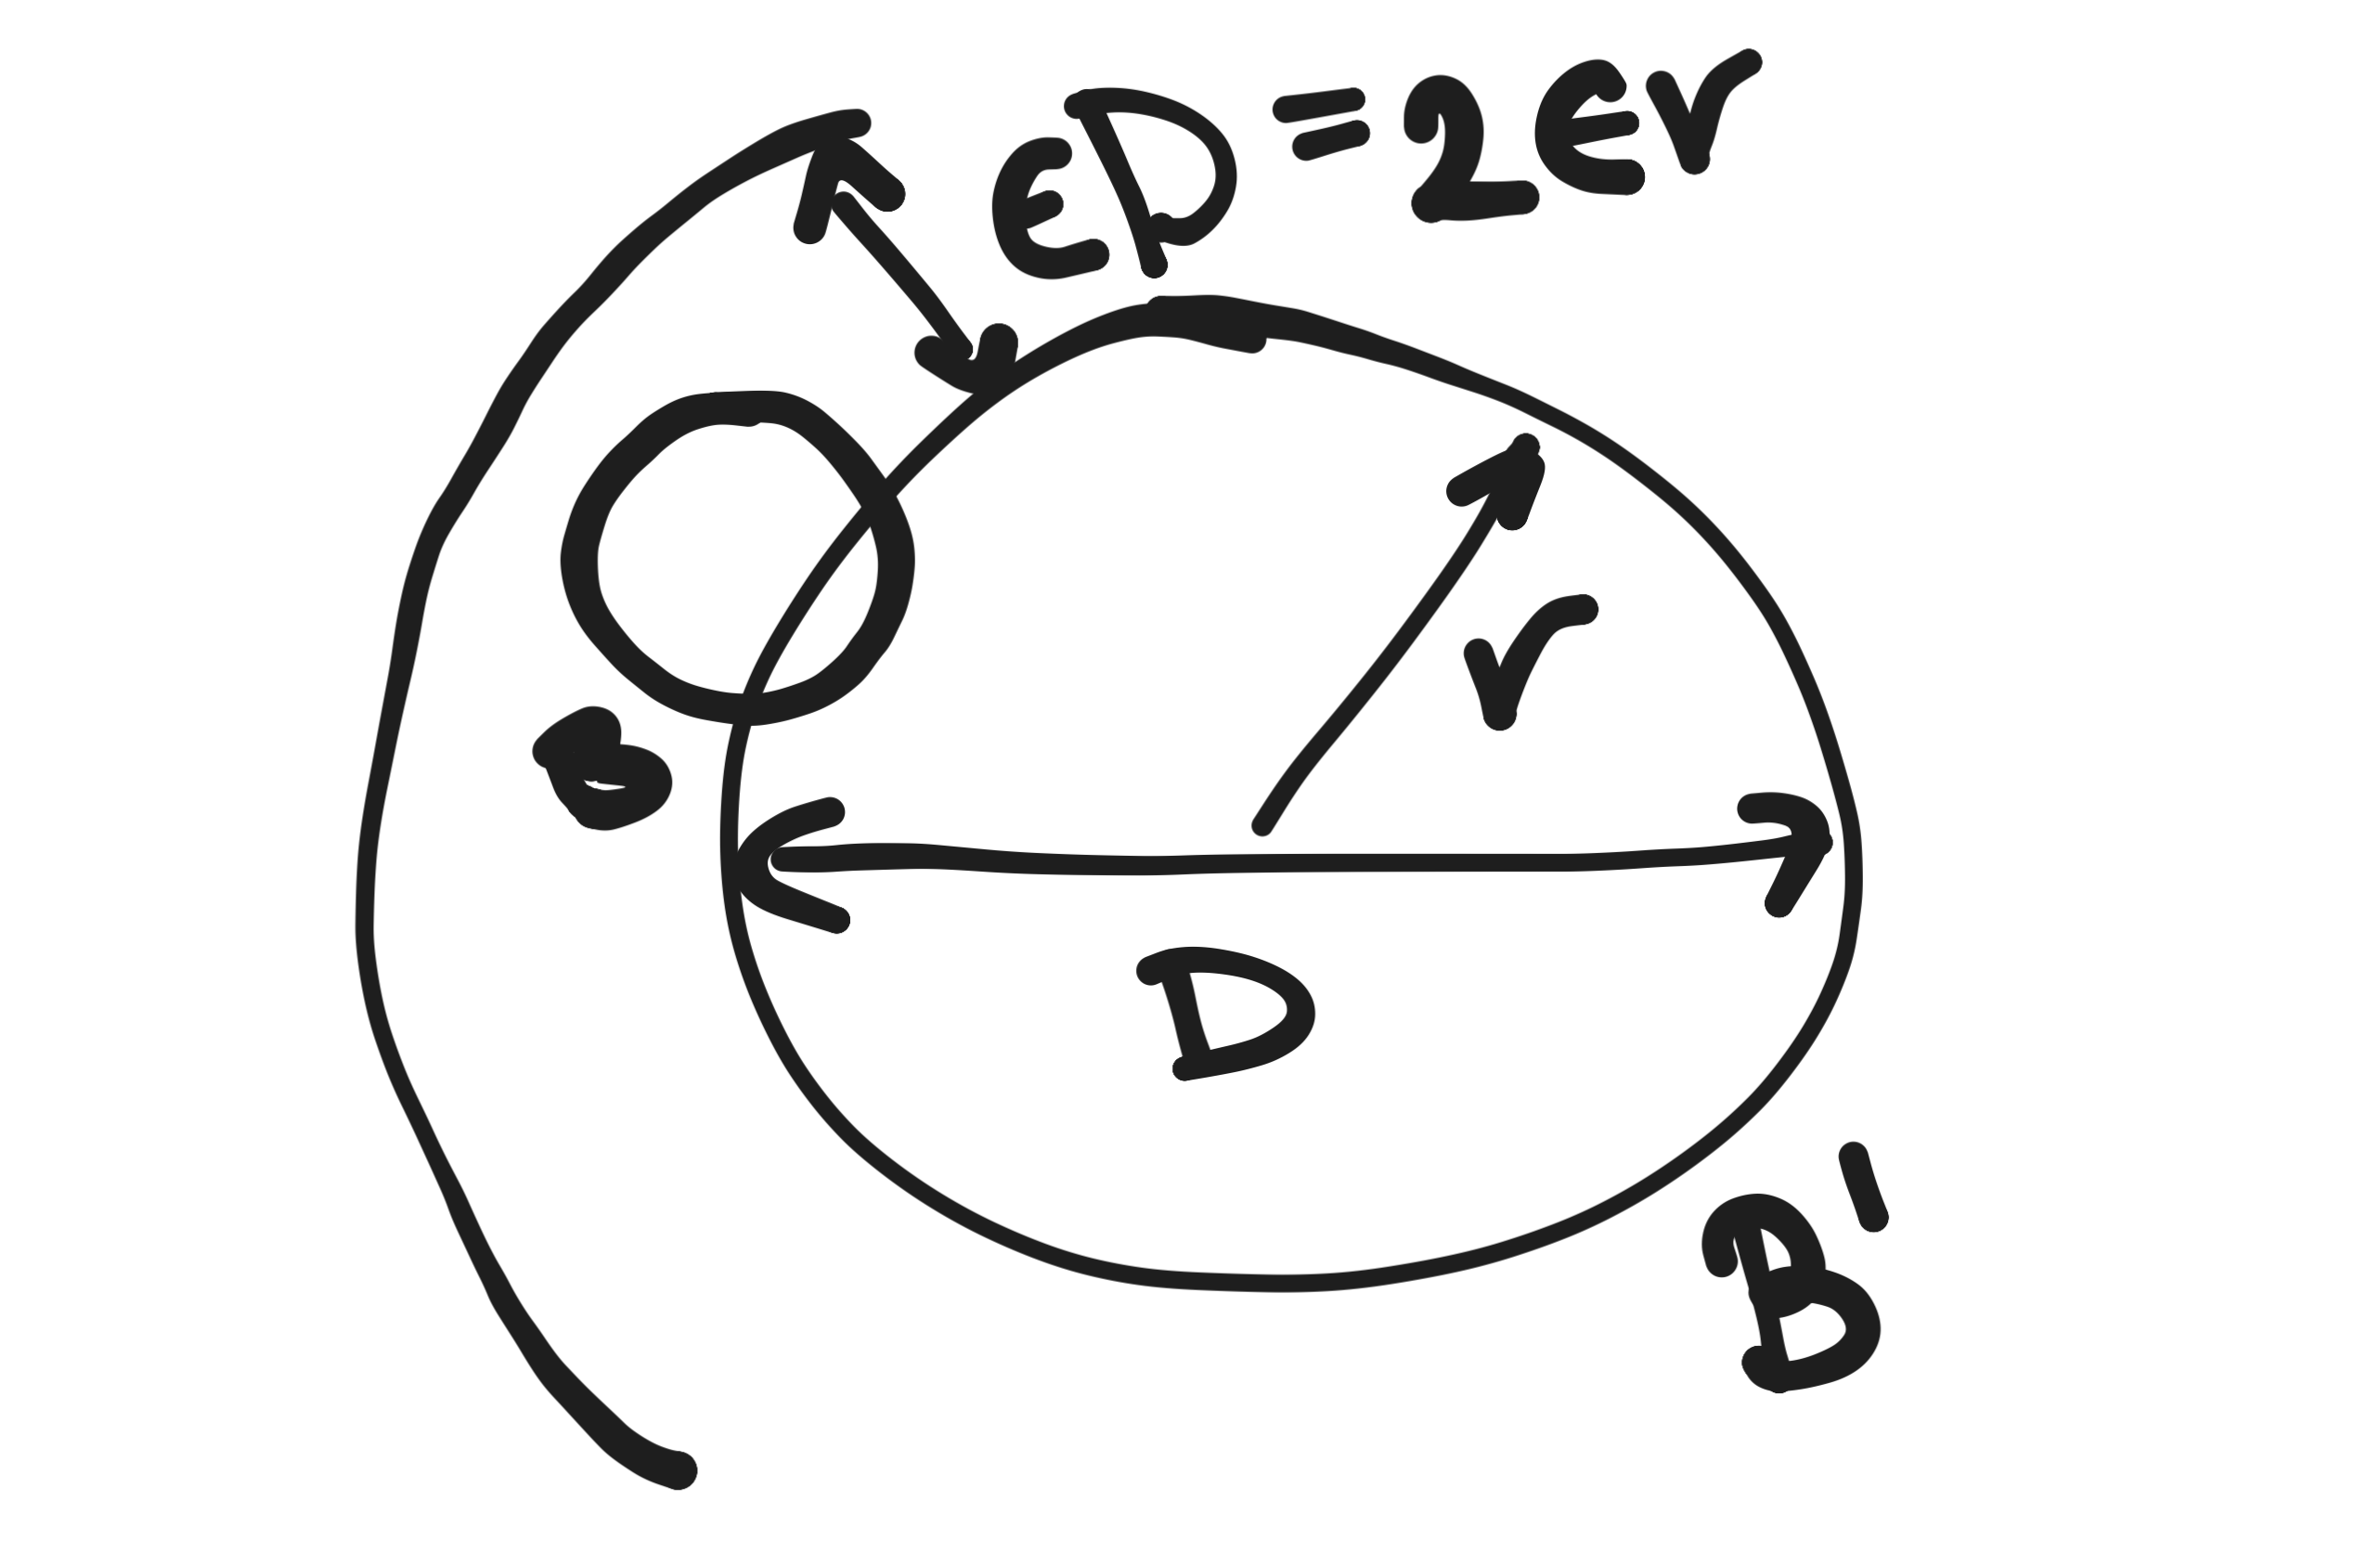
\includegraphics[scale=0.1]{Vitali.png}
\end{center}
\vspace{1ex}
\textbf{Remark:} This is a generalised version of the proof from the book
"Measure theory and fine properties of functions" where it is done for the
smallest integral case $\epsilon = 2$. The generalised proof shows the reason
why the final dilatation is $5 = 1+2\epsilon$, but actually it is true for
dilatation $>3$ and the smallest such integer is 4. An interesting question is
whether there is continuity and can we take a limit and get this result also
for 3.

\vspace{2ex}

There are also more substantial covering results, crucial for extension 
theorems, measure differentiation and characterisation of rectifiable sets.
Their proofs usually occupies a dozen of pages and are deeply analytic, primarily
involving the extensive rewrite of inequalities and introduction of different
constants. I initially intended to revise them for greater clarity, but after
several failed attempts, when I had to modify constants and propagate the change
back over multiple pages, I decided it was best to simply reference them here.
Full proofs are available in \cite{evans_gariepy} and in \cite{giovanni_alberti}.


\vspace{2ex}
\textbf{Besicovitch’s Covering Theorem:} \textit{There exists a constant $N_n$, depending
only on the dimension $n$ with the following property:}

\vspace{1ex} \textit{
If $\mathcal{F}$ is any collection of non-degenerated closed balls in
$\mathbb{R}^n$ with
\[\sup\{\textnormal{diam}\,B\,|\,B\in\mathcal F\}<\infty\]
and $A$ is the set of centers of balls in $\mathcal F$, then there $N_n$
countable collections $\mathcal{G}_1,\ldots,\mathcal{G}_{N_n}$ of disjoint
balls in $\mathcal{F}$ such that
\[A\subseteq\bigcup_{i=1}^{N_n}\bigcup_{B\in\mathcal{G_i}}B\]}

\vspace{2ex}
\textbf{Definition:} \textit{A cover of $A$ by a family $B$ is called \textbf{fine}
if for any $x\in A$ we can find a covering set from $B$ of arbitrary small
diameter.}

\vspace{2ex}
\textbf{Filling open sets with balls theorem:} \textit{Let $\mu$ be a Borel measure on
$\mathbb{R}^n$, and $\mathcal{F}$ any collection of non-degenerated closed balls.
Let $A$ denote the set of centers of the balls in $\mathcal F$. Assume
\[\mu(A)<\infty\]
and $\mathcal F$ is a fine cover of $A$. Then for each open set $U\subseteq\mathbb{R}^n$, there
exists a countable collection $\mathcal G$ of disjoint balls in $\mathcal F$ such that
\[\bigcup_{B\in\mathcal G} B\subseteq U\]
and
\[\mu\left((A\cap U)\setminus\bigcup_{B\in\mathcal G}B\right)=0.\]}

\vspace{2ex}
\textbf{Whitney's extension theorem:}\textit{
Let $C\subseteq \mathbb{R}^n$ be a closed set and $f:C\rightarrow\mathbb R$,
$d:C\rightarrow\mathbb{R}^{n*}$ be continuous functions. We shall use notions}
\begin{align*}
    &R(y,x)=\frac{f(y)-f(x)-d(x)(y-x)}{|x-y|},\quad\forall x,y\in C, x\neq y \\
    &\rho_k(\delta)=\sup\{|R(x,y)|\, |\, 0<|x-y|\leq\delta, x, y\in K\}
\end{align*}
\textit{if we suppose that for every compact $K\subseteq C$}
\[
\rho_K(\delta)\rightarrow 0\text{ as }\delta\rightarrow 0
\]

\textit{Then there exists a function $\overline f\in\mathcal{C}^1(\mathbb{R}^n,\mathbb{R})$
and $D\overline f|_C=d$.}

\vspace{2ex}
\textbf{Definition:} \textit{For a function $f:X\rightarrow Y$ between metric spaces we can
define its \textbf{Lipschitz constant} $\text{Lip}(f) = \textnormal{inf}\{L\in
\mathbb{R}\,|\,d(f(x),f(y))\leq Ld(x,y) \forall x,y\in X\}$}

\vspace{2ex}
\textbf{Lipschitz function extension theorem:} \textit{Let $X$ be a metric space,
$A\subseteq X$ and $f:A\rightarrow\mathbb{R}$. Then there exists a Lipschitz
function $\overline f:X\mapsto\mathbb{R}$ such that $\textnormal{Lip}(f)=\textnormal{Lip}
(\overline f)$ and $\overline f|_A=f$.}

\vspace{1ex}
Let's set
$L=\text{Lip}(f)$. Then we define
\[\overline f(x) = \text{inf}_{y\in A}(f(y)+Ld(x,y)\]
By the definition, for all $x\in A$, $\overline f(x)\leq f(x)$ as in particular
we can chose $y=x$.
Furthermore, for all $a,b\in A$ and $x\in X$, we have an inequality for a
Lipschitz function $f(b)-f(a)\leq Ld(b,a)\leq Ld(b,x)+Ld(a,x)$ and thus we have
\[ f(a)+Ld(a,x)\geq f(b)-Ld(b,x)\] 
and if we apply an infinum over a, we have $\overline f(x)\geq f(b)-L(b,x)$ and
if $x\in A$ we can chose $b=x$ and we have an inequality in the other direction
and thus the equality $\overline f(x)=f(x)$.

\vspace{1ex}
Now we check the Lipschitz constant
%\begin{align*}
%
%\end{align*}

\vspace{1ex}
\textbf{Consequence:} \textit{Let $X$ be a metric space, $A\subseteq X$ and
$f:A\rightarrow\mathbb{R}^n$. Then there exists a Lipschitz
function $\overline f:X\mapsto\mathbb{R^n}$ such that $\overline f|_A=f$}

\vspace{1ex}
Let's set $\overline f = (\overline f_i)_i$ extension by coordinate functions. 

\vspace{1ex}
\textbf{Remark:} I considered extending the theorem to vector-valued
functions, but I could only prove it for the maximum norm.

\subsection{Differentiation of Radon measure and Radon-Nikodym Theorem}

\vspace{2ex}
\textbf{Definition:} \textit{Let $\mu$ and $\nu$ be Radon measures on $\mathbb{R}^n$.
Then we can define upper and lower derivatives of $\nu$ by $\mu$ by
\begin{align*}
    &\overline D_\mu\nu(x) =
    \left\{\begin{array}{rcl}
        \limsup_{r\rightarrow0}\frac{\nu(B(x,r))}{\mu(B(x,r))} & \textnormal{if }\mu(B(x,r))>0\textnormal{ for all }r>0\\
        +\infty & \quad\textnormal{if }\mu(B(x,r))=0\textnormal{ for some }r>0
    \end{array}\right.\\
    &\underline D_\mu\nu(x) =
    \left\{\begin{array}{rcl}
        \liminf_{r\rightarrow0}\frac{\nu(B(x,r))}{\mu(B(x,r))} & \textnormal{if }\mu(B(x,r))>0\textnormal{ for all }r>0\\
        +\infty & \quad\textnormal{if }\mu(B(x,r))=0\textnormal{ for some }r>0
    \end{array}\right.
\end{align*}
If $\overline D_\mu\nu(x)=\underline D_\mu\nu(x)<+\infty$ then we say that $\nu$
is \emph{differentiable} with respect to $\mu$ at x and we write
\[D_\mu\nu(x)=\overline D_\mu\nu(x)=\underline D_\mu\nu(x)\]
}

\vspace{1ex}
\textbf{Definition:} \textit{Let $\mu$ be Radon measure and $\nu$ be a vector measure on
$\mathbb{R}^n$. Then we define a derivatives as
\[
    D_\mu\nu(x) =
    \left\{\begin{array}{rcl}
        \lim_{r\rightarrow0}\frac{\nu(B(x,r))}{\mu(B(x,r))} & \textnormal{if }\mu(B(x,r))>0\textnormal{ for all }r>0\\
        +\infty & \quad\textnormal{if }\mu(B(x,r))=0\textnormal{ for some }r>0
    \end{array}\right.
\]
}

\vspace{1ex}
While vector-valued measures are defined later, it suffices to know that they
are set functions with values in vector spaces that satisfy a particular version
of sigma-additivity.

\vspace{2ex}
\textbf{Differentiating measures theorem:} \textit{Let $\mu$ and $\nu$ be Radon
measures on $\mathbb{R}^n$. Then
\begin{itemize}
    \item $D_\mu\nu$ exists and is finite $\mu$-a.e.
    \item $D_\mu\nu$ is $\mu$-measurable
\end{itemize}
}

\vspace{2ex}
\textbf{Remark:} This is a brilliant version of the proof of Radon-Nikodym
Theorem by von Neumann, that will suffice for representing vector measures.

\vspace{1ex}
\textbf{Radon-Nikodym Theorem:} \textit{Let $\mu$ and $\nu$ be finite measures
on $(\Omega, \mathcal F)$ then there exists a non-negative measurable function
$f$ and a $\mu$-null set $B$ such that
\[\nu(A) = \int_Af\,d\mu+\nu(A\cap B)\]
for each $A \in \mathcal F$.
}

\vspace{1ex}
\textbf{Proof:} Let $\pi=\mu+\nu$ and consider $T(f)=\int fd\nu$. Then for
every $f\in L^2(\pi)$ we have $f\in L^1(\nu)$ and since measures are finite
$f\in L^1(\pi)$ and thus in $L^1(\nu)$, then
\[|T(f)|=|\int f\,d\nu|\leq\|f\|_{L^2(\nu)}\|1\|_{L^2(\nu)}\leq C\|f\|_{L^2(\pi)}\]
where $C$ is a constant. Thus $T$ is a continuous operator on $L^2(\pi)$ and by
Reisz representation theorem for Hilbert spaces we find a function $h\in L^2(\pi)$
such that
\[T(f)=\int f\,d\nu=\int fh\,d\pi\]
Now consider the following sets
\[N=\{h<0\},\quad M=\{0\leq h<1\},\quad B=\{h\geq 1\}\]
Then
\[0\geq\int_N h\,d\pi=\int\chi_N h\,d\pi=\nu(N)\geq 0\]
Thus we have $\nu(N)=0$ and since $h<0$ on $N$ and $\int h\,d\mu=0$ we have
$\mu(N)=0$ also.

\vspace{1ex}
Now let's study $B$. We have
\[\nu(B)=T(\chi_B)=\int_Bh\,d\mu+\int_B h\,d\nu\geq\nu(B)+\mu(B)\]
thus $\mu(B)=0$.

For the last let we set $M_n=\{0\leq h\leq1-1/n\}$ and from representation of
$T$ with $h$ we have $\int(1-h)f\,d\nu=\int hf\,d\mu$ and why apply it to
\[\nu(M_n)=\int\frac{\chi_{M_n}}{1-h}(1-h)\,d\nu=\int h\frac{\chi_{M_n}}{1-h}\,d\mu\]

Let $f=\frac{h}{1-h}$ then by applying monotone convergence and recalling that
$\mu(B)=\mu(N)=0$ we have
\[\nu(M\cap A)=\int_A f\,d\mu\]

Finally for all $A\in\mathcal F$ we have
\[\nu(A)=\nu(A\cap N)+\nu(A\cap M)+\nu(A\cap B) = \int_A f\,d\mu+\nu(A\cap B)\]

\vspace{2ex}
\textbf{Corollary:} If $\mu >> \nu$, then $\nu(A)=\int_A f\,d\mu$

\vspace{1ex}
It's evident since $\mu(B)=0\Rightarrow\nu(B)=0$ then. 

\vspace{2ex}
\textbf{Remark:} If $\mu$ and $\nu$ are Radon measures, then $f=D_\mu\nu$.

\vspace{2ex}
\textbf{Corollary:}
This gives us a representation of a vector valued measure $\mu$ as $\mu=f\,|\mu|$.
And we can define the integration with respect to such measure as
\[
\int g\,d\mu = \int g\cdot f\,d|\mu|
\]

\vspace{2ex}
Beyond representation of measure (or continuous linear forms), we can view this
process from another angle. If we associate to a linear continuous
form to a shape, then function $f$ describes certain geometric properties of
that shape. We will explore one such example in the last section.
